% !TeX spellcheck = hu_HU
\documentclass[12pt,a4paper]{article}
\usepackage[utf8]{inputenc}
\usepackage{cmap}
\usepackage[T1]{fontenc}
\usepackage[magyar]{babel}
\usepackage{amsmath}
\usepackage{amsfonts}
\usepackage{amssymb}
\usepackage{graphicx}

\usepackage{outlines}
\usepackage{hyperref}

\hyphenpenalty=10000

\def\ojoin{\setbox0=\hbox{$\bowtie$}%
  \rule[-.02ex]{.25em}{.4pt}\llap{\rule[\ht0]{.25em}{.4pt}}}
\def\leftouterjoin{\mathbin{\ojoin\mkern-5.8mu\bowtie}}
\def\rightouterjoin{\mathbin{\bowtie\mkern-5.8mu\ojoin}}
\def\fullouterjoin{\mathbin{\ojoin\mkern-5.8mu\bowtie\mkern-5.8mu\ojoin}}

\def\tef{\to\to}

\begin{document}

\begin{center}
	\huge
	Adatbázisok I\\
	\vspace{1mm}
	\LARGE
	Előadás és gyakorlat jegyzet\\
	\vspace{5mm}
	\large
	Készült Szalai-Gindl János Márk előadásai\\
	és Vörös Péter gyakorlatai alapján\\
	\vspace{5mm}
	Sárközi Gergő, 2021-22-2. félév\\
	Nincsen lektorálva!
\end{center}

\tableofcontents

\pagebreak

\section{Bevezetés}

\begin{outline}
	\1 Adatbázis: Database Management System által kezelt adatok együttese
	\1 DBMS feladatai:
		\2 Adatbázis létrehozása, adatbázis séma definiálása
		\2 Adatok lekérdezése, módosítása (hatékonyan)
		\2 Nagyméretű adatok hosszú időn történő tárolása
		\2 Autentikáció és meghibásodás ellen védelem
		\2 Egyszerre több felhasználó egyidejű hozzáférésének biztosítása
	\1 Több adatbázist egy adattárház (middleware) fog össze
\end{outline}

\section{Relációs adatmodell}

\begin{outline}
	\1 Adatmodell: információ/adatok leírására szolgáló jelölés
		\2 Adatok struktúrája
		\2 Adatokon végezhető műveletek
		\2 Adatokra vonatkozó megszorítások (pl. unique)
	\1 Legfontosabb adatmodellek: relációs, félig strukturált (XML)
	\1 Adatok 2D-s táblákban (relációkban) vannak
		\2 Egy reláció az sorok halmaza, ennek a halmaznak neve: előfordulás
		\2 Halmaz $\implies$ nem számít a sorrend, egy sor max egyszer szerepelhet
	\1 Reláció fejrészében attribútumok vannak
		\2 Relációséma: attribútumok halmaza; adatelemek adatainak formája
		\2 attribútumok sorrendje nem fix, nevük alapján hivatkozhatók
		\2 attribútumok meghatározzák az értékkészletet
	\1 Adatbázis: relációk halmaza
	\1 Egy sor elemei: mezők (komponensek)
		\2 Csak atomi értékeket vehetnek fel: szám, szöveg, referencia, stb.
\end{outline}

\pagebreak

\section{Relációs algebra}

\begin{outline}
	\1 Algebra: műveletek és atomi operandusok
		\2 Eredmény: reláció
		\2 Operandusok: konstansok, változók (relációkból)
	\1 Monoton operátor: egy reláción értelmezett operátor akkor monoton, ha bármely argumentumrelációhoz egy újabb sort hozzávéve az eredmény tartalmazza az összes eddigi sort, és esetleg újabbakat is
\end{outline}

\subsection{Megszorítások}

\begin{outline}
	\1 Megjegyzés: algebrai műveletek lejjebb vannak, de kellenek ide
	\1 Relációra vonatkozó megszorítás: $R = \emptyset$ vagy $R \subseteq S$
		\2 Kifejezőkészségük azonos, pl. $R$ sorai részhalmaza $S$ sorainak
	\1 Hivatkozási épség megszorítás: ha itt megjelenik, ott is meg kell
		\2 Kifejezés: $\Pi_A(R) \subseteq \Pi_B(S)$
	\1 Kulcs: attribútumok halmaza egy kulcs, ha a reláció bármely (mostani és jövőbeli) előfordulásában nincs két olyan sor, amelyek a kulcs összes attribútumának értékein megegyeznek.
		\2 Példa: (a, b) kulcs: $\sigma_{R.a=S.a \wedge R.b = S.b \wedge R.c \ne S.c}(R\times S) = \emptyset$
		\2 Aláhúzással jelöljük (általában?)
\end{outline}

\pagebreak

\subsection{Algebrai műveletek}

\begin{outline}
	\1 Projekció, vetítés: attribútumok szűkítése, jelölés: $\Pi_{A,B}(R)$
	\1 Szelekció, kiválasztás: feltétel alapján sorok szűrése
		\2 Jelölés: $\sigma_{A=a \wedge C=d}(R)$
		\2 Minden tag 1 vagy 2 attribútumból áll (vagy 2, vagy 1 és 1 konstans)
		\2 A tagokban ezek a műveletek lehetnek: $=, <, >, \ne, \le, \ge$
		\2 A tagokat ezek kapcsolhatók: $\lnot, \wedge, \lor$
	\1 Unió, metszet, különbség
		\2 Feltétel: operandusok attribútumai megegyeznek
	\1 Descartes-szorzat, jelölés: $R \times S$
		\2 Azonos nevű attribútumok a reláció nevét kapják prefixnek
		\2 Asszociatív (szabadon zárójelezhető), kommutatív (felcserélhető)
	\1 Átnevezés: $\rho_{S(C,D,E)}(R)$ vagy $\rho_S(R)$
	\1 Théta-összekapcsolás: $R \bowtie_F S \Leftrightarrow \sigma_F (R \times S)$ \;
	(ahol $F$ egy feltétel)
		\2 Példa: $R \bowtie_{R.A = S.A} S$
		\2 Kommutatív
		\2 Asszociatív, ha a feltétel nem használ olyan attribútumot, ami a "távolabbi" (csak megfelelő zárjelezés esetén elérhető) relációból származik
			\3 $E_1 \bowtie_{F_1} (E_2 \bowtie_{F_2} E_3) \equiv (E_1 \bowtie_{F_1} E_2) \bowtie_{F_2} E_3$\\
			ha $attr(F_1) \subseteq attr(E_1) \cup attr(E_2)$\\
			és \;$attr(F_2) \subseteq attr(E_2) \cup attr(E_3)$
	\1 Egyen-összekapcsolás, equi join:
		\2 Théta-összekapcsolás, ahol egyenlőség a feltétel
	\1 Természetes összekapcsolás: Théta, F= minden azonos attribútum egyezik
		\2 Jelölés: $R \bowtie S$
		\2 Alternatíva: Théta-összekapcsolás, majd közös attribútumokból 1
		\2 Kommutatív, asszociatív (mindig)
\end{outline}

\pagebreak

\section{Relációs algebrai lekérdezések optimalizációja}

\begin{outline}
	\1 Ekvivalens lekérdezések: tetszőleges előfordulás esetén is azonos eredmény
	\1 Lépések (mindezt egy fán használjuk):
		\2 Műveletek szétbontása (pl. konjunkció, összekapcsolás)
			\3 Természetes összekapcsolásból Descartes-szorzat és kiválasztás
		\2 Műveletek a levélhez közel helyezése (minél előbbre)
		\2 Projekciók behelyezése (nem szükséges oszlopok levágása)
			\3 Akkor nagy a nyereség, ha az oszlopok vannak külön-külön fájlban tárolva (nem pedig a sorok)
			\3 Nem kötelező kiválasztás elé: elég kiválasztás után, de összekapcsolás előtt
		\2 Természetes és théta összekapcsolásokra cserélni, amit lehet
	\1 Diszjunkció bonyolultabb, mint a konjunkció
	\1 Van arra példa, hogy egy kiválasztást először felfelé kell csúsztatni, hogy
	aztán le lehessen tolni.
\end{outline}

\subsection{Műveletek optimalizációja}

\begin{outline}
	\1 Projekció sorozat: $X \subseteq Y \implies \Pi_X(\Pi_Y(E)) \equiv \Pi_X(E)$
	\1 Kiválasztás és feltételek...
		\2 konjunkciója: $\sigma_{F1}(\sigma_{F2}(E)) \equiv \sigma_{F1 \wedge F2}(E)$
		\2 diszjunkciója: $\sigma_{F1}(E) \cup \sigma_{F2}(E) \equiv \sigma_{F1 \lor F2}(E)$
	\1 Kiválasztás elé projekció beillesztése:\\
	$Y = attr(F) \cup X \implies \Pi_X(\sigma_F(E)) \equiv \Pi_X(\sigma_F(\Pi_Y(E)))$
	\1 Kiválasztás és Descartes-szorzat/összekapcsolás:
		\2 Legyen $\Delta$ vagy $\times$ vagy $\bowtie$
		\2 Ha $F=F_1 \wedge F_2$ és $attr(F_i) \subseteq attr(E_i)$\\
		Akkor $\sigma_F(E_1 \Delta E_2) \equiv \sigma_{F_1} (E_1) \Delta \sigma_{F_2} (E_2)$
		\2 Ha $F=F_1 \wedge F_2$ és $attr(F_1) \subseteq attr(E_1)$ de $attr(F_2) \not \subseteq attr(E_i)$\\
		Akkor $\sigma_F(E_1 \Delta E_2) \equiv \sigma_{F_2}(\sigma_{F_1} (E_1) \Delta E_2)$
\pagebreak
	\1 Projekció és Descartes-szorzat/összekapcsolás:
		\2 Legyen $\Delta$ vagy $\times$ vagy $\bowtie$
		\2 Ha $X=Y \cup Z$ és $Y \subseteq attr(E_1)$ és $Z \subseteq attr(E_2)$
		\2 Akkor $\Pi_X(E_1 \Delta E_2) \equiv \Pi_Y(E_1) \Delta \Pi_Z(E_2)$
	\1 Kiválasztás és halmazműveletek: disztributív\\
	Legyen $\Delta$ vagy $\cap$ vagy $\cup$ vagy $\setminus$:
	$\sigma_F (E_1 \Delta E_2) \equiv \sigma_F(E_1) \Delta \sigma_F(E_2)$
	\1 Projekció és unió disztributivitás: $\Pi_X(E_1 \cup E_2) \equiv \Pi_X (E_1) \cup \Pi_X (E_2)$
\end{outline}

\subsection{Optimalizációra példa}

\begin{outline}
	\1 Feladat: Kik azok a 20 évesek, akik moszkvai kiadású könyvet kölcsönöztek?
		\2 Személy(név, kor, város, ISBN)
		\2 Könyv(cím, író, ISBN, ár)
		\2 Kiad(k-cím, k-író, város, ország)
\end{outline}

\begin{figure}[h!]
	\centering
	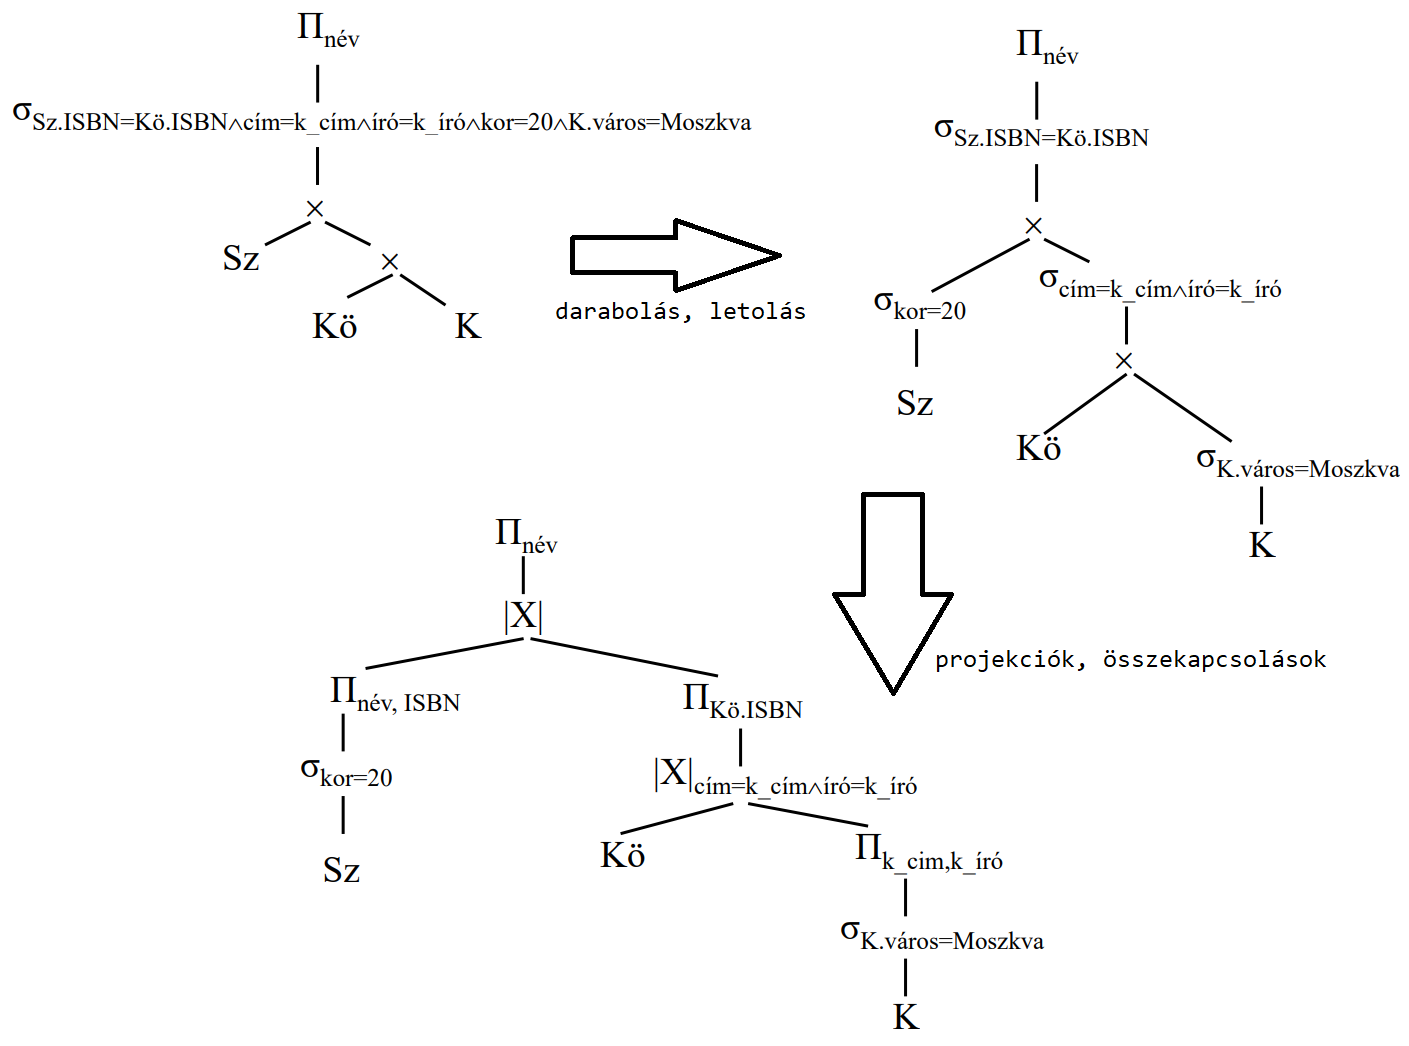
\includegraphics[width=0.9\linewidth]{relalg-optimize-short}
\end{figure}

\pagebreak

\section{SQL bevezetés}

\begin{outline}
	\1 Magas szintű nyelv: "hogyan" helyett "mit"-et írjuk le
	\1 Adatbázis kezelő optimalizál: kitalálja a leggyorsabb végrehajtási módot
	\1 Itt már multihalmaz van: lassú mindig kitörölni az ismétlődést
\end{outline}

\subsection{Lekérdezés jelentése}

\begin{outline}
	\1 Kezdjük a FROM záradékban megadott relációval
	\1 Alkalmazzuk a WHERE záradékban megadott kiválasztási feltételt
	\1 Levetítjük az eredményt a SELECT-ben megadott oszlopokra
\end{outline}

\subsection{SQL érdekességek}

\begin{outline}
	\1 SELECT *
	\1 SELECT név AS sör; SELECT ár*300 AS árForint
	\1 SELECT 'konstans' as valami (pl. adattárházban integráció miatt)
	\1 WHERE alapműveletek: AND, OR, NOT, $=,<>,<,>,<=,>=$
	\1 WHERE attribútum (NOT) LIKE minta
		\2 Mintában \%: 0 vagy több akármilyen karakter
		\2 Mintában \_: pontosan egy akármilyen karakter
		\2 Mintában bármilyen más karakter: önmagát jelenti
	\1 WHERE attr BETWEEN x AND y (ahol x kötelezően kisebb, mint y)
	\1 Több táblából lekérdezés: FROM után több tábla
		\2 Ezután duplikált attribútum nevek neve: TÁBLA.OSZLOP
	\1 Azonos táblából többször: FROM tábla t1, tábla t2
	\1 Alapból multihalmaz, ha ne: SELECT DISTINCT
\end{outline}

\pagebreak

\subsection{NULL értékek}

\begin{outline}
	\1 Mezők NULL értéket is tartalmazhatnak
	\1 Lehetséges jelentés: hiányzik, értelmetlen
	\1 SQL 3 értékű logikát használ: TRUE, FALSE, UNKNOWN
		\2 Legyen TRUE=1, FALSE=0, UNKNOWN=0.5
		\2 Ekkor AND=MIN, OR=MAX, NOT(x)=1-x
	\1 NULL-al hasonlítás (akár NULL-t): eredmény UNKNOWN
		\2 Helyesen: IS (NOT) NULL
	\1 Egy sor WHERE-ben UNKNOWN, akkor nem kerül be az eredménybe
\end{outline}

\subsection{Alkérdések}

\begin{outline}
	\1 FROM és WHERE záradékban SELECT-FROM-WHERE-t is használhatunk
		\2 FROM esetén az ideiglenes táblának nevet kell adni általában
	\1 Egy sort visszaadó alkérdések
		\2 Konstans értéknek lehet kezelni
		\2 Általában csak egy oszlopa van
		\2 Futásidejű hiba keletkezik, ha több sor van
	\1 Tábla rendes kérdésben és alkérdésben is be van húzva: oszlopnév alapból a legközelebbi FROM-ra vonatkozik (azaz az alkérdésre)
	\1 Alkérdéses műveltek:
		\2 Tartalmazás: sor (NOT) IN alkérdés
		\2 Alkérdés (nem) üres: (NOT) EXISTS alkérdés
			\3 Korrelált alkérdés: minden sorra külön lefut, mert függ tőlük
		\2 Halmazműveletek: INTERSECT, UNION, MINUS (=EXCEPT)
			\3 Nem multihalmaz, hanem halmaz szemtikát halmaz
			\3 Hogy mégis multihalmaz legyen: <UNION/...> ALL
		\2 ANY, ALL: pl. x > ANY(alkérdés); x <> ALL(alkérdés)
\end{outline}

\pagebreak

\subsection{Összekapcsolás (join)}

\begin{outline}
	\1 Emlékeztető: $NULL \ne NULL$
	\1 Természetes összekapcsolás: a NATURAL JOIN b
		\2 SQL optimalizál: nincs SELECT-elve az oszlop $\implies$ nem működik
		\2 Önmagával: $NULL \ne NULL$, tehát $NULL$-os sorok eltűnnek
	\1 Descartes-szorzat: a CROSS JOIN b (ugyan az, mint a vessző: a, b)
	\1 Théta-összekapcsolás: a JOIN b ON aa = bb
		\2 Ugyan az, mint az INNER JOIN
		\2 Ugyan az, mint: a, b WHERE aa = bb
\end{outline}

\section{SQL haladó}

\subsection{Összekapcsolás (join)}

\begin{outline}
	\1 Félig összekapcsolás (SEMI JOIN, '$\ltimes$'): olyan természetes összekapcsolás, ami csak az első relációból veszi az attribútumokat
		\2 SELECT R.* FROM R WHERE EXISTS(... R.A = S.A)
	\1 Anti összekapcsolás (ANTI JOIN, '$\rhd$'): $R \rhd S \equiv R \setminus R \ltimes S$
		\2 SELECT R.* FROM R WHERE NOT EXISTS(... R.A = S.A)
	\1 Külső összekapcsolás:
		\2 SQL-ben: R <típus> (OUTER) JOIN S (ON ...)
			\3 Típus: LEFT ($\leftouterjoin_C$), RIGHT ($\rightouterjoin_C$), FULL ($\fullouterjoin_C$ or $ _L\bowtie_{R\;C}$)
			\3 Vagy NATURAL, vagy ON szerepel (vagy semmi): kizáróak
		\2 Lógó sor: eredmény része, de nincs hozzárendelt sor másik relációban
			\3 Külső összekapcsolás lényege: ilyen sorokat megőrzi
			\3 Ilyenkor a hiányzó oszlopok NULL értékű lesznek
\end{outline}

\begin{figure}[h!]
	\centering
	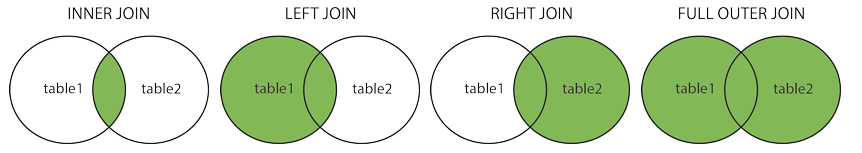
\includegraphics[width=0.7\linewidth]{joins}
\end{figure}

\pagebreak

\subsection{Összesítések (aggregációk)}

\begin{outline}
	\1 SELECT záradékban alkalmazhatjuk egy-egy oszlopra
	\1 SUM, AVG, COUNT, MIN, MAX
	\1 Összesító függvényen belül DISTINCT: COUNT(DISTINCT ár)
	\1 NULL érték nem számít: mintha nem is lenne ott a sor
	\1 Üres halmaz eredménye: NULL, kivéve COUNT: ott 0
	\1 Ha GROUP BY nélkül van: mintha az egész reláció egy csoport lenne
\end{outline}

\subsection{Csoportosítás (grouping)}

\begin{outline}
	\1 WHERE utén záradék: GROUP BY oszlop
	\1 SELECT sör, AVG(ár) FROM x GROUP BY sör;
	\1 SELECT-ben csak bizonyos dolgok lehetnek:
		\2 Összesítések, amelyek így csoportonként kiértékelődnek
		\2 Attribútumok, amik alapján GROUP BY-t csináltunk
	\1 Csoport szűrés: HAVING ("megfelelője": WHERE)
		\2 Értelemszerűen meg van szorítva, mint a SELECT 
\end{outline}

\subsection{Sorba rendezés}

\begin{outline}
	\1 ORDER BY = ORDER BY ASC; másik: ORDER BY DESC
\end{outline}

\pagebreak

\subsection{Adatbázis módosítások}

\begin{outline}
	\1 Nem query: nem ad vissza eredményt
	\1 Insert, Update, Delete
	\1 Data Manipulation Language
\end{outline}

\subsubsection{Beszúrás}

\begin{outline}
	\1 INSERT INTO <tábla> VALUES (...)
		\2 Itt minden oszlopnak értéket kell adni
	\1 Tábla neve után megadhatók az attribútumok:
		\2 INSERT INTO sör(név, ár) VALUES ('Bud', 100)
		\2 Így a sorrendet "lokálisan" definiáljuk, nem kell emlékezni
		\2 A hiányzó attribútumok default (NULL/beállított) értéket kapnak
	\1 Több sor beszúrása: INSERT INTO <reláció> (alkérdés);
\end{outline}

\subsubsection{Törlés}

\begin{outline}
	\1 DELETE FROM <reláció> (WHERE ...)
	\1 Nincs WHERE: összes sor törlése
		\2 Alternatíva: TRUNCATE TABLE <név> (ez séma módosítás féleség)
	\1 Két lépésben hajtódik végre:
		\2 Először törlendő sorok kijelölése, majd kijelölt sorok kitörlése
		\2 Emiatt determinisztikus: nem számít melyik tűnik el előbb
\end{outline}

\subsubsection{Módosítás}

\begin{outline}
	\1 UPDATE <reláció> SET oszlop1=v1, oszlop2=v2, ... [WHERE ...]
\end{outline}

\pagebreak

\subsection{Adatbázis sémák}

\begin{outline}
	\1 Data Definition Language
	\1 Létrehozás: CREATE TABLE <név> (<elemek, megszorítás listája>);
		\2 Elem: <név> <típus> [sor megszorítás] [DEFAULT <érték>]
		\2 Megszorítás: CONSTRAINT <név\_FK> <FK szintaxis lejebb>
	\1 Törlés: DROP TABLE <név>;
\end{outline}

\subsubsection{Típusok}

\begin{outline}
	\1 Szám: INT=INTEGER, REAL=FLOAT
		\2 Tizedesvessző: . (pont)
	\1 Szöveg: CHAR(n) (mindig n), VARCHAR(n) (legfeljebb n)
		\2 VARCHAR2(n): Oracle valami, $\sim$ VARCHAR
		\2 Aposztrófok közé kell rakni
		\2 Két aposztróf = egy igazi aposztróf (escape)
	\1 DATE, megadás: DATE 'yyyy-mm-dd'
		\2 Gyakon megadás: TO\_DATE('2000.01.01', 'YYYY.MM.DD')
	\1 TIME, megadás: TIME 'hh:mm:ss' vagy TIME 'hh:mm:ss.tizedmp'
\end{outline}

\subsubsection{Tábla módosítás}

\begin{outline}
	\1 ALTER TABLE <név> ....
		\2 DROP COLUMN/CONSTRAINT <név>
		\2 ADD <név> <típus> [megszorítások, stb]
		\2 MODIFY <meglévő név> <új típus> [megszorítások, stb]
	\1 Oszlopot nem lehet töröli, ha van hozzá CONSTRAINT
\end{outline}

\pagebreak

\subsection{Megszorítások}

\begin{outline}
	\1 Adatelemek közötti kapcsolat
	\1 Adatbázis rendszer tartja fel őket
	\1 Relációs algebrában: egy lekérdezés értéke legyen pl. üres vagy részhalmaz
	\1 Gyakori megszorítás: NOT NULL
\end{outline}

\subsubsection{Kulcsok}

\begin{outline}
	\1 Attribútum vagy attribútum lista lehet kulcs
		\2 Egy esetén: create table-ben, attribútum sora végén is lehet
		\2 Több esetén: csak az attribútum lista után lehet
	\1 Relációnak nem lehet két sora, amiben megegyeznek
	\1 PRIMARY KEY vagy UNIQUE
		\2 PRIMARY KEY-ből csak 1db lehet, nem lehet NULL
		\2 UNIQUE-ból több is lehet, lehet NULL
	\1 Oracle SQL: nincs AUTO INCREMENT, helyette hack:\\
	INSERT INTO x(y) VALUES ((SELECT MAX(y)+1 FROM x))
\end{outline}

\subsubsection{Idegen kulcsok, hivatkozási épség megszorítás}

\begin{outline}
	\1 Relációs algebrában: $\Pi_{beer}(Serve) \subseteq \Pi_{name}(Beer)$
	\1 Megadható attribútum után vagy séma végén
		\2 név típus REFERENCES reláció(attribútum)
		\2 FOREIGN KEY (attribútumok...) REFERENCES reláció (attribútumok...)
	\1 Csak kulcs (PRIMARY KEY / UNIQUE) attribútumokon működik
	\1 Sértheti: beszúrás vagy a másik oldalon törlés/módosítás
		\2 Rossz beszúrást csak egyféleképpen kezel az SQL: nem engedi
		\2 Rossz törlés/módosítás kezelése:
			\3 Default: szerintem ezt jelenti: nem engedi a módosítást (RESTRICT)
			\3 Továbbgyűrűzés: másik táblában is töröljük/módosítjuk sor(ok)at
			\3 Set NULL: másik táblában NULL értéket kap
			\3 ... KEY ... ON [UPDATE/DELETE] [SET NULL / CASCADE]
\end{outline}

\pagebreak

\subsubsection{Attribútum alapú (érték-alapú) megszorítás}

\begin{outline}
	\1 Egy adott oszlopra vonatkozik a megszorítás, annak értékeit ellenőrzi
	\1 Csak beszúrásnál, módosításnál van végrehajtva
		\2 Azaz törlésnél nem
		\2 Azaz foreign-key féle koncepció nincsen
	\1 Megadás: attribútum után CHECK(feltétel)
		\2 Alapból csak a saját attribútumra hivatkozhatunk
		\2 Alkérdés segítségével bármi hivatkozható
\end{outline}

\subsubsection{Sor-alapú megszorítás}

\begin{outline}
	\1 Sor mezei közötti kapcsolatot definiál
	\1 Csak beszúrásnál és módosításnál van végrehajtva
	\1 Megadás: reláció séma után CHECK(feltétel)
		\2 Saját relációban bármelyik attribútumra hivatkozhatunk
		\2 Alkérdés segítségével bármilyen reláció hivatkozható
\end{outline}

\subsubsection{Globális megszorítás}

\begin{outline}
	\1 Adatbázissémához tartozik (nem pedig relációhoz)
	\1 Bármira hivatkozhat (tetszőleges tábla, tetszőleges oszlop)
	\1 Minden módosítás előtt (insert, update, delete) ellenőrizve van
		\2 Adatbázis rendszer optimalizálhat: nem nézi meg mindig
	\1 CREATE ASSERTION név CHECK (feltétel)
\end{outline}

\pagebreak

\subsection{Trigger}

\begin{outline}
	\1 Kód végrehajtódik, amikor egy esemény történik (pl. sor beszúrása)
	\1 Más név: ECA szabály (event-condition-action)
	\1 Példa: beszúrás visszautasítása helyett (foregin key miatt), beszúrhatunk egy sort a másik táblába is automatikusan (pl. NULL értékkel kiegészítve)
	\1 CREATE TRIGGER név ... (nagyon sok lehetőség van)
	\begin{verbatim}
		CREATE TRIGGER SörTrig
		BEFORE INSERT ON Felszolgál
		REFERENCING NEW ROW AS ÚjSor
		FOR EACH ROW
		WHEN (ÚjSor.sör NOT IN (SELECT név FROM Sörök))
		INSERT INTO Sörök(név) VALUES(ÚjSor.sör);
	\end{verbatim}
\end{outline}

\pagebreak

\subsection{Tranzakciók}

\begin{outline}
	\1 Egység, amit osztatlanul kell végrehajtani
	\1 Lehet lekérdezés és/vagy módosítás
	\1 Minden SQL utasítás az: 1 elemes tranzakció
	\1 Perzisztálni kell: végrehajtás közben rendszerhiba $\implies$ ne legyen baj
	\1 Részei:
		\2 Konkurenciakezelő: atomicitás megvalósítása, versenyhelyzetek kizárása
		\2 Naplózás- és helyreállítás-kezelés: tranzakciók tartóssága (perzisztencia)
	\1 Műveletek végrehajtási sorrendje fontos (race condition)
	\1 Valamilyen szinten párhuzamosítva van
\end{outline}

\subsubsection{ACID tranzakciók}

\begin{outline}
	\1 Atomicity: vagy az összes, vagy semelyik utasítás hajtódik végre
	\1 Consistency: adatbázis megszorítások megőrződnek
	\1 Isolation: úgy tűnik, mintha a folyamatok egymás után futnának le
	\1 Durability: befejeződött tranzakció módosításai nem vesznek el
	\1 Opcionálisan gyengébb feltételek is megadhatóak
		\2 pl. osztott adatbázisoknál kötelező
\end{outline}

\subsubsection{SQL utasítások}

\begin{outline}
	\1 COMMIT: tranzakció módosításai megőrződnek
	\1 ROLLBACK: tranzakció abortál, összes utasítás vissza van görgetve
		\2 0-val való osztás, stb. automatikus ezt eredményezi
\end{outline}

\pagebreak

\subsubsection{Elkülönítési szintek}

\begin{outline}
	\1 Egy tranzakció milyen állapotot láthat (részeredmények, stb.)
	\1 Négy elkülönítési szint (ACID-ban I betű finomhangolása)
	\1 SET TRANSACTION ISOLATION LEVEL <level>
		\2 A pillatnyi connection-re állítja be
	\1 SERIALIZABLE (magyarul: sorbarendezhető)
		\2 Tranzakciók nem befolyásolják egymást, nincs átfedés.
	\1 REPEATABLE READ
		\2 Csak COMMIT-olt adatot látni, külön-külön olvasásoknál extra sorok megjelenhetnek (ha közben van módosítás). Sorok soha nem módosulhatnak, nem tűnhetnek el.
		\2 Többletsor neve: fantomsor, fantomadat.
	\1 READ COMMITTED
		\2 Csak COMMIT-olt adatot látni, de a tranzakción belül minden művelet lehet, hogy más adaton dolgozik: közben lehet módosítás.
		\2 "Nem ismételhető olvasás"
	\1 READ UNCOMMITTED
		\2 A nem COMMIT-olt változtatásokat is látja (piszkos adatokat)
\end{outline}

\pagebreak

\subsection{Nézettáblák}

\begin{outline}
	\1 Nézettáblát alaptáblákból és más nézettáblákból definiáljuk
	\1 Virtuális nézettábla: nem tárolódik adat, csak a relációt megadó lekérdezés
	\1 Materializált nézettábla: maga az adat tárolódik
		\2 Ha sokat lekérdezzük a nézettáblát, akkor gyorsabb lehet
		\2 Minden módosítás esetén frissül automatikusan, ami idő
			\3 Beállítható: X időn belül vagy periodikus frissítés
			\3 Azaz nem kötelező a legfrissebb adatnak benne lennie
		\2 Előnye új táblához képest:
			\3 Adatbáziskezelő helyettünk frissíti
			\3 Lekérdezés optimalizáció akár ki tudja használni ezeket a táblákat
	\1 CREATE (MATERIALIZED) VIEW <név> AS <lekérdezés>
	\1 Állítólag pár egyszerű módosítást nézettáblán keresztül is lehet csinálni
	\1 NEM nézettábla, hanem másolás: CREATE TABLE <név> AS <lekérdezés>
\end{outline}

\subsection{Indexek}

\begin{outline}
	\1 Adatszerkezet, amivel egy-egy relációt gyorsabban lekérdezhetünk egy/több attribútum alapján
	\1 Megvalósítás lehet hash table, de általában bináris fa
	\1 SQL-ben deklarálás
		\2 Nincs szabvány/standard megoldás
		\2 CREATE INDEX <IndexNév> ON Tábla(Oszlop)
		\2 CREATE INDEX <IndexNév> ON Tábla(Oszlop1, Oszlop2, ...)
	\1 Használatuk: automatikus, csak a megfelelő attribútum alapján szűrjünk
	\1 Hangolás: indexek bevezetése gyorsíthat, de nem feltétlenül jó
		\2 Indexek mellett: felgyorsítja a lekérdezéseket
		\2 Indexek ellen: módosítások lassulnak; indexeket is frissíteni kell
		\2 Menete: query load $\implies$ indexek készítése $\implies$ hatás vizsgálata
\end{outline}

\pagebreak

\section{SQL jogosultságkezelés}

\begin{outline}
	\1 9 féle jogosultság van, némelyik oszlop szinten is megadható
	\1 Pár relációra vonatkozó jogosultság:
		\2 SELECT (lehet, hogy csak adott attribútumra vonatkozik)
		\2 INSERT (lehet, hogy csak adott attribútumra vonatkozik)
		\2 DELETE
		\2 UPDATE (lehet, hogy csak adott attribútumra vonatkozik)
	\1 Jogosultságokat lehet adni még:
		\2 Nézettábla (virtuális és materializált) lekérdezés/módosítás
		\2 Relációhoz index, trigger, nézettábla létrehozása
	\1 Jogosultsági azonosító (authorization ID)
		\2 Általában a bejelentkezési név
		\2 Egy másik: PUBLIC
	\1 Jogosultságok megadása
		\2 Általunk létrehozott dolgokra minden jogunk megvan
		\2 GRANT <jogosultságok...> ON <reláció/valami> TO <JogAzonosítók...>
		\2 ... WITH GRANT OPTION: jogosultságot kapó tovább is adhatja
	\1 Jogosultságok visszavonása
		\2 REVOKE <jogosultságok...> ON <reláció/valami> FROM <JogAzonosítók...>
		\2 Több helyről kapták a jogot $\implies$ megmaradhat utána is
		\2 REVOKE-hoz meg kell adni egyet:
			\3 CASCADE: a továbbadott jogosultságokat is megvonjuk
			\3 RESTRICT: addig nem működik a REVOKE, amíg érvényben van még továbbadott jog
		\2 REVOKE GRANT OPTION ... is létezik
\end{outline}

\pagebreak

\subsection{Grant diagrammok}

\begin{outline}
	\1 Jogosultság gráf
	\1 Pontok: felhasználó/jogosultság/grant option-e/tuladonos-e
		\2 Külön pontnak számít: UPDATE ON R és UPDATE ON R(a)
		\2 AP nevű pont: A azonosítójú P jogát jelenti
		\2 AP*: P-hez van grant jog
		\2 AP**: tulajdonosságból származik a jog
	\1 $X \to Y$ él: X pontot használtuk Y megadására
	\1 Alapvető szabály:
		\2 Legyen C és X felhasználó (akár azonos)
		\2 Legyen Q egy jogosultság, amit P magába foglal (akár azonos)
		\2 C-nek addig van joga Q-hoz, amíg vezet XP**-ból az egyikbe út:\\
		CQ, CQ*, CQ**
	\1 Gráf frissítéskor: pont nem érhető el egy **-ból se $\implies$ törölni kell
\end{outline}

\pagebreak

\section{Relációs adatbázis tervezés}

\begin{outline}
	\1 Minden adat egyetlen relációban: kényelmes, de sok a felesleges adat
		\2 Rossz tárolási hatékonyság
		\2 Ellentmondásossá válhat (nem változtatjuk meg mindenhol az adatot)
	\1 Jobb megoldás: felhasználói eset fogalmait, kapcsolatait modellezni kell
	\1 Jelölés: X,Y,Z attribútum halmaz; A,B,C pedig attribútum
\end{outline}

\subsection{Kulcsok}

\begin{outline}
	\1 K szuperkulcs R relációra, ha K funkcionálisan meghatározza R attribútumait
	\1 K kulcs R-en, ha K szuperkulcs, de egyetlen valódi részhalmaza sem az
	\1 Azaz például $user\_id,address$ szuperkulcs, de $user\_id$ kulcs
	\1 Kulcs megkapása: paraszti ésszel vagy FF-ek alapján következtetjük ki
\end{outline}

\subsection{Funkcionális függőségek (FF)}

\begin{outline}
	\1 Redundancia: egy/több oszlopból ki tudunk következtetni egy harmadikat
	\1 Funkcionális függőség ($X \to Y$): ha két sor megegyezik $X$ összes attribútumán, akkor $Y$-jain is
	\1 Jobboldalak szétvágása (ff): $X \to A_1A_2... \Leftrightarrow X \to A_1 \wedge X \to A_2 \wedge ...$
\end{outline}

\subsubsection{Armstrong-axiómák 1}

\begin{outline}
	\1 Reflexivitás: ha $Y \subseteq X \subseteq R$ akkor $X \to Y$ (triviális függőség)
	\1 Bővítés: $X \to Y$ akkor tetszőleges $Z \subseteq R$ esetén $XZ \to YZ$
	\1 Tranzitivitás: $X \to Y \wedge Y \to Z \implies X \to Z$
	\1 Felhasználás példa:
		\2 Feladat: ha $X \to Y$ és $XY \to Z$ akkor $X \to Z$
		\2 $X \to Y$ bővítés után $X \to XY$
		\2 $X \to XY$ és $XY \to Z$ reflexivitás miatt $X \to Z$
\end{outline}

\pagebreak

\subsubsection{Lezárás}

\begin{outline}
	\1 Y lezártja ($Y^+$): attribútum halmaz, ami következik $Y$-ból
		\2 Azaz: $\forall A \in Y^+: Y \to A$
	\1 Ha Y szuperkulcs, akkor $Y^+$ az összes attribútum lesz
	\1 Kiszámítás: iteratívan
		\2 Első lépés: $Y^+ = Y$
		\2 Indukció: ha $X \subseteq Y^+$ és $X \to A$, akkor $A$-t belerakjuk $Y^+$-ba
		\2 Iteráció vége: ha utolsó lépésben $Y^+$ nem változott
	\1 Bizonyítás: $B \in Y^+ \implies Y \to B$
		\2 Indukcióval (valószínűleg nem kéri számon)
	\1 Bizonyítás: nem lett egy $B$ sem kihagyva
		\2 Indirekt módon (valószínűleg nem kéri számon)
\end{outline}

\subsubsection{Összes következmény FF, szétbontás, FF projekció}

\begin{outline}
	\1 Motiváció: egy relációsémát több sémára bontunk
	\1 Ha tudunk attribútumokat és FF-eket, akkor az attribútumok részhalmazán milyen FF-ek lesznek? (normalizálás)
	\1 Példa: eredeti: $AB \to C, C \to D, D \to A$\\
	ABC részhalmazon teljesül: $AB \to C$ és $C \to A$
	\1 Exponenciális algoritmus:
		\2 Minden lehetséges X halmazhoz számítsuk ki $X^+$-ot
		\2 Függőségekhez adjuk hozzá $\forall X \to A$-t, ahol $A \in X^+ \setminus X$
		\2 Dobjuk ki $XY \to A$-t, ha $X \to A$ is teljesül
		\2 Végül csak azokat az FF-eket nézzük, amikben csak a projektált attribútumok vannak
		\2 Trükk: $\emptyset^+ = \emptyset$ és $R^+ = R$
		\2 Trükk: $X^+ = R \wedge X \subseteq Y \implies Y^+ = R$
\end{outline}

\pagebreak

\subsubsection{FF-ek geometriaia reprezentációja}

\begin{outline}
	\1 Minden pont egy lehetséges előfordulás (olyan sorhalmaz, ami létezhetne)
	\1 Minden FF egy régió: előfordulások részhalmaza, amire igaz
	\1 Triviális FF: a régió a teljes tér
	\1 Több FF is teljesül: régiók metszete
	\1 Legyen $A \to B$ és $B \to C$. Ekkor az $A \to C$ régi tartalmazza a két másik régió metszetét, de bővebb nála (valódi tartalmazás, nem egyenlőség).
\end{outline}

\begin{figure}[h!]
	\centering
	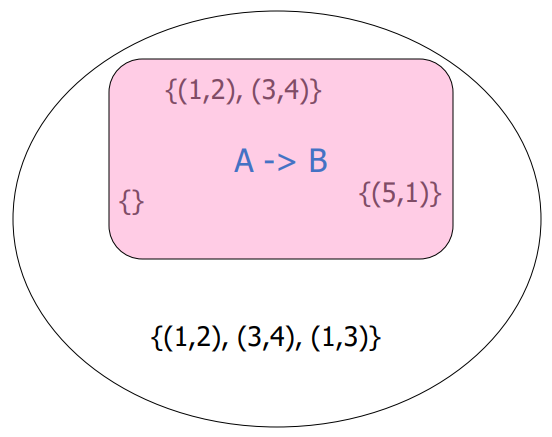
\includegraphics[width=0.5\linewidth]{FF-geometriai-reprezentáció}
\end{figure}

\pagebreak

\subsection{Relációs sémák tervezése}

\subsubsection{Relációk felbontása}

\begin{outline}
	\1 Bemenet: $R(A_1,...,A_n)$; kimenet: $S(B_1,...,B_m),T(C_1,...,C_k)$ relációk
		\2 $\{A_1,...,A_n\} = \{B_1,...,B_m\} \cup \{C_1,...,C_k\}$
		\2 $S = \Pi_{B1,...,Bm}(R)$ és $T=\Pi_{C1,...,Ck}(R)$
	\1 Cél: veszteségmentes felbontás: $r = \Pi_{R1}(r) \bowtie ... \bowtie \Pi_{Rk}(r)$
		\2 $r$: egy $R$ sémájú reláció
		\2 $\Pi_{Ri}(r)$: $r$ sorai az $Ri$ attribútumaira (több van!) projektálva
		\2 Példa nem veszteségmentesre: $ABC$-t $AB$-re és $BC$-re bontjuk,\\
		de $B$ oszlop minden eleme azonos, $A$ és $C$ elemei viszont nem
	\1 Cél: funkcionális függőségek megőrzése
		\2 Nem mindig sikerül
	\1 Cél: redundancia, anomáliák (felsorolva alul) megszüntetése
		\2 (Nem mindig sikerül)
		\2 Módosítási: nem mindenhol módosul az adat (redundancia miatt)
		\2 Törlési anomália: olyan is törlődik, aminek nem kéne\\
		pl. ha senki nem szeret egy sört, akkor tudjuk, hogy ki gyártja?
		\2 Beszúrási: nem tudunk beszúrni, mert olyan adatot kéne megadni, ami nincs értelmezve egy adott esetben (pl. kedvenc söre anyámnak)
\end{outline}

\pagebreak

\subsubsection{Boyce-Codd normálforma (BCNF)}

\begin{outline}
	\1 $R$ reláció BCNF formában van, ha $\forall X \to Y$ nemtriv FF-re $X$ szuperkulcs
		\2 Nemtriviális: $Y$ nem része $X$-nek
		\2 Szuperkulcs: tartalmaz kulcsot (akár ő maga egy kulcs)
	\1 Veszteségmentes, de FF-ek nem feltétlenül őrződnek meg, de FF-ek okozta anomália nem lehet benne
	\1 BCNF-re való felbontás
		\2 Legyen $R$ reláció, $F$ FF-ek halmaza
		\2 Van-e olyan $X \to Y$ FF, ami sérti a BCNF-et?
			\3 Elég $F$-et végignézni: ha $F^+$-ban valami sérti, akkor $F$-ben is
			\3 Hogyan: $X^+$-ban nincs minden attribútum $\implies$ nem szuperkulcs
		\2 $R$ dekomponálása $X \to Y$ alapján
			\3 $R_1 = X^+$ és $R_2 = R - (X^+ - X)$
			\3 Projektáljuk $F$-beli FF-eket a két új relációra
			\3 Példa ($F$: név $\to$ cím, név $\to$ kedvenc, kedvelt $\to$ gyártó)
				\4 Bemenet: Főnökök(név, cím, kedveltSörök, gyártó, kedvenc)
				\4 név $\to$ cím: R1(név, cím, kedvenc) R2(név, kedvelt, gyártó)
				\4 Ez még mindig nem BCNF: $R2$-t ketté kell szedni
	\1 Belátása, hogy a BCNF-re való felbontás veszteségmentes
		\2 Tranzitivitás féleség: ha $R_1,...,R_k$ egy veszteségmentes felbontása $R$-nek,
		és $S_1,S_2$ egy veszteségmentes felbontása $R_1$-nek,
		akkor $S_1,S_2,R_2,...,R_k$ egy veszteségmentes felbontása $R$-nek
		\2 Tehát csak azt kell belátni, hogy a dekomponálás veszteségmentes
		\2 Ez pedig triviális (legalábbis az EA diákon ez a magyarázat)
\end{outline}

\pagebreak

\subsubsection{Chase-teszt vesztességmentességhez}

\begin{outline}
	\1 Megmondja, hogy veszteségmentes-e egy felbontás
	\1 Példa eset:
		\2 Eredeti reláció: $R(A,B,C,D)$
		\2 FF-ek: $F = \{A \to B, B \to C, CD \to A\}$
		\2 Felbontás: $R_1(A,D)$, $R_2(A,C)$, $R_3(B,C,D)$
	\1 Egy táblázatot használ az algoritmus:
		\2 Oszlopok az eredeti $R$ oszlopai
		\2 Sorok: minden $R_i$-hez egy sor
		\2 Cellák: oszlop $R_i$ része akkor ismert ($x$) egyébként ismeretlen ($x_i$)
	\1 A cél az általános sor ($a,b,c,d$) kialakítása. Az FF-ek használjuk fel.
		\2 Két egyenlővé teendő szimbólum közül...
			\3 Egyik index nélküli: másik is azt az értéket kapja
			\3 Mindkét indexes: a kisebbik indexet kapja mindkettő
		\2 A lecserélt szimbólum minden előfordulását le kell cserélni
	\1 Egyszer nem feltétlenül elég végigmenni az FF-eken: tetszőleges sorrendben vettük végig őket, ami lehet, hogy nem optimális. Addig kell újra-újra lefuttatni az "algoritmust", amíg változik az eredmény.
		\2 Ha megkaptuk az általános sort, akkor biztosan veszteségmentes.\\
		Ismételni csak akkor kell, ha nem kaptuk meg.
\end{outline}

\begin{figure}[h!]
	\centering
	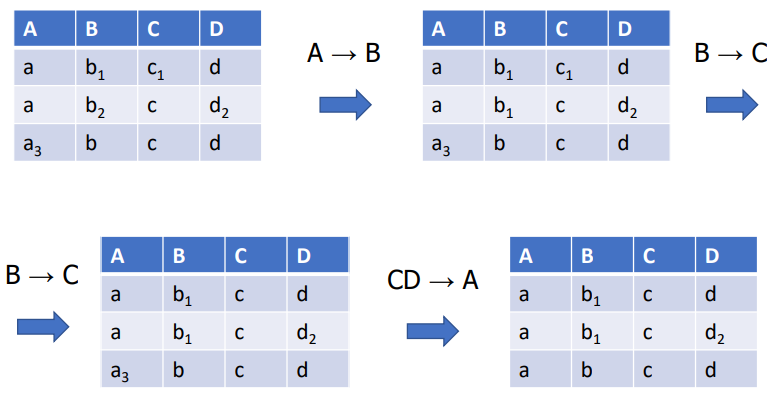
\includegraphics[width=0.7\linewidth]{Chase-teszt}
\end{figure}

\pagebreak

\subsubsection{Minimális bázis}

\begin{outline}
	\1 Bázis: $F$-fel ekvivalens FF halmaz
	\1 Minimális bázis
		\2 Jobb oldalon mindig csak egy attribútum van
		\2 Bármely függőség elhagyása esetén már nem bázis
		\2 Bármely bal oldal csökkentése esetén már nem bázis
	\1 Minimális bázis létrehozása algoritmikusan: (legyen $F$ az FF-ek halmaza)
		\2 Kezdetben $G = \emptyset$
		\2 Függőségek $X \to A$ alakra hozása (jobboldalak szétvágása):\\
		$\forall \; X \to Y \in F, \; A \in Y \setminus X:$ az $X \to A$ FF-eket tegyük $G$-be
		\2 Nem szükséges függőségek elhagyása:\\
		$X \to A \in G$ elhagyása, ha $X \to A$ következik $(G \setminus \{X \to A\})$-ból
		\2 Baloldalak minimalizálása:\\
		Ha $X \to A \in G$ és $\exists B \in X: A \in (X \setminus \{B\})^+$ ($G$ szerint),
		azaz $G$ ekvivalens marad: $G$-ben $X \to A$ lecserélése $(X \setminus \{B\}) \to A$-ra
\end{outline}

\subsubsection{Harmadik normálforma (3NF)}

\begin{outline}
	\1 Motiváció: BCNF felbontáskor veszíthetünk el függőségeket
		\2 Példa: AC,BC sémákkal nem lehet az $AB \to C$ egy FF
	\1 Veszteségmentes, megőrzi az FF-eket, de anomália maradhat
	\1 Prím (elsődleges) attribútum: legalább egy kulcsnak az eleme
	\1 Definíció: $X \to A$ nem triviális FF csak akkor sérti meg 3NF-et, ha $X$ nem szuperkulcs és $A$ nem prím
		\2 BCNF-től eltérés: FF akkor is szabályos, ha jobboldal prím
	\1 Minimális bázisból 3NF-re bontás
		\2 Minimális bázis minden FF-jének bal- és jobboldalának uniója egy séma,
		pl.: $X \to A$ esetén XA egy séma
		\2 Ha az így kapott sémák között nincs szuperkulcs, akkor egy extra séma:
		valami, ami egy kulcs az R reláción
			\3 Ez a veszteségmentességhez kell
	\1 Helyesség belátása:
		\2 Függőségeket megőrizni a minimális bázis miatt
		\2 Veszteségmentes, amit a Chase-tesztel be lehet látni
\end{outline}

\subsection{Többértékű függőségek}

\subsubsection{Többértékű függőség (TÉF)}

\begin{outline}
	\1 Jelölés: $X \tef Y$
	\1 $X$ minden értékei esetén $Y$ értékei függetlenek az $R \setminus X \setminus Y$ értékeitől
		\2 Azaz ha két sorban $X$ értékei egyeznek $\implies$ $Y$ értékei felcserélhetők
	\1 Példa: Alkesz(név, tel, kedveltSör): telefonszám független a sörtől
		\2 név $\tef$ tel és név $\tef$ kedveltSör
		\2 Azaz egy adott névhez tartozó telefonok, sörök minden kombinációja létezik a sorok között
	\1 Triviális TÉF: $X \tef Y$ ahol $Y \subseteq X$ vagy $X \cup Y = R$ \;\; ($X,Y \subseteq R$)
\end{outline}

\subsubsection{Többértékű függőség szabályok}

\begin{outline}
	\1 Minden FF egyben TÉF: $X \to Y \implies X \tef Y$
		\2 Ha két sor egyezik $X$-en, akkor $Y$-on; felcserélve ugyan azt kapjuk
	\1 Komplementálás: $X \tef Y \implies X \tef (R \setminus X \setminus Y)$
		\2 $X$ megegyezik, akkor mindegy: $Y$-t cseréljük fel / minden mást
	\1 FF-ekkel ellentétben a jobboldalak nem darabolhatók szabadon
	\1 Bővíthetőség: ha $X \tef Y$ és $V \subseteq W$ akkor $XW \tef YV$
	\1 Tranzitivitás: $X \tef Y \wedge Y \tef S \implies X \tef S \setminus Y$
\end{outline}

\pagebreak

\subsubsection{Negyedik normálforma (4NF)}

\begin{outline}
	\1 Motiváció: TÉF-ek okozta redundanciát BCNF nem szünteti meg
	\1 4NF: TÉF-eket dekomponáláskor FF-ként kezeljük\\
	(kulcs kereséskor a TÉF-ek nem számítanak)
	\1 $R$ akkor van 4NF-ben, ha $\forall$ nemtriv. $X \tef Y$ esetén $X$ szuperkulcs
	\1 $R$ 4NF-ben van $\implies$ BCNF-ben is (fordítva nem igaz)
		\2 Minden FF, ami BCNF-et megsérti, az a 4NF-et is megsérti
	\1 4NF dekompozíció, ha $X \tef Y$ sérti 4NF-et: (hasonló BCNF-hez)\\
	$R_1 = XY$ és $R_2 = R \setminus (Y \setminus X)$
\end{outline}

\subsubsection{TÉF-ek és FF-ek együttes következtetése}

\begin{outline}
	\1 Feladat: egy TÉF, FF halmazból következik-e egy adott TÉF/FF?
	\1 Megoldás: tabló, Chase ötlet kiterjesztése
	\1 Chase-teszt kiterjesztése
	\1 TÉF esetén írjuk be a szükséges sorokat, hogy a TÉF igaz legyen
	\1 Vagy ha $X \tef Y$ bizonyítása a feladat, akkor kezdjünk 2 $X$-ben egyező és $R \setminus X$-ben különböző sorral és lássuk be (FF-ek és TÉF-ek segítségével), hogy a két sor megegyezik
	\1 Nem sikerült felfognom a példák levezetését, így ezen témakör jegyzete hiányos.
\end{outline}

\pagebreak

\section{Egyed-kapcsolat modell, E/K diagram}

\subsection{Cél, motiváció}

\begin{outline}
	\1 Adatbázisséma felvázolása
	\1 Később relációs adatbázissémává alakítható
	\1 Tervezést segíti (főbb részek felvázolása)
\end{outline}

\subsection{Alafogalmak}

\begin{outline}
	\1 Egyed
	\1 Egyedhalmaz (téglalap): mint OOP-ben egy osztály
		\2 Csak struktúrát tekintünk, végezhető műveleteket nem
		\2 Értéke: hozzá tartozó egyedek halmaza
	\1 Attribútum (ovális): atomi érték (szám, szöveg) (tömb/rekord NEM!)
		\2 Össze vannak kötve egyedhalmazzal
	\1 Kapcsolat (rombusz): 2 (bináris) vagy több egyedhalmazt köt össze
		\2 Értéke a kapcsolathalmaz: sorok halmaza, minden sorban a kapcsolatban résztvevő egyedhalmazokból van 1-1 darab
\end{outline}

\pagebreak

\subsection{Kapcsolatokról bővebben}

\subsubsection{Kapcsolatok típusai}

\begin{outline}
	\1 Általában bináris kapcsolatról beszélünk most
	\1 Sok-sok: mindkét adathalmaz egyedei 0/1/sok másik egyedhez kapcsolódhatnak
		\2 Jelölése: sima vonal
	\1 Sok-egy: (jelölése: "egy" oldalon háromszög nyíl van)
		\2 Első egyedhalmaz minden eleme legfeljebb egyhez kapcsolódnak
		\2 Második egyedhalmaz elemei 0, 1 vagy több egyedhez kapcsolódhatnak
	\1 Egy-egy: minden entitáns legfeljebb egy másikhoz kapcsolódik
		\2 Jelölése: mindkét végén háromszög nyíl
	\1 "Legfeljebb" helyett "pontosan" egy: lekerekített nyíl ($-\triangleright$ helyett $\to$)
	\1 Alternatív jelölés: él címkézése [a,b] intervallummal (sok=n)
\end{outline}

\begin{figure}[h!]
	\centering
	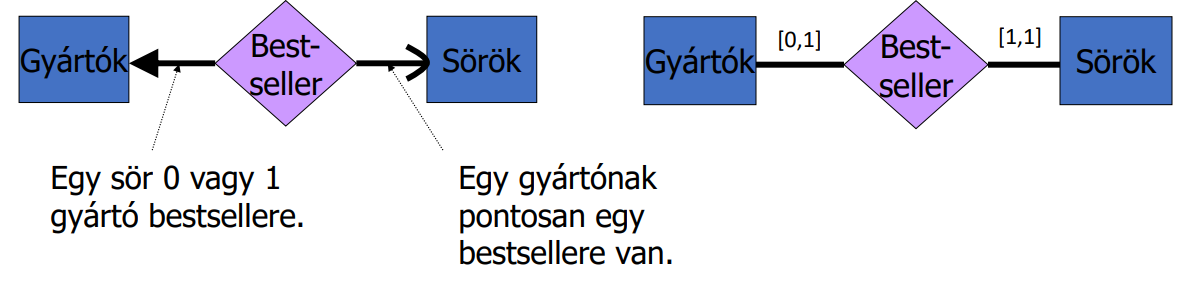
\includegraphics[width=0.5\linewidth]{EK-kapcsolat}
\end{figure}

\subsubsection{Kapcsolatok attribútumai}

\begin{outline}
	\1 Az attribútum a kapcsolatban álló egyedhalmazok együttes tulajdonsága
	\1 Jelölés: simán hozzákötünk egy attribútumot a kapcsolathoz
	\1 Alternatív jelölés: egyedhalmaz bevezetése és vastag háromszöges nyíllal rámutatunk a kapcsolatból
\end{outline}

\begin{figure}[h!]
	\centering
	\includegraphics[width=0.45\linewidth]{EK-kapcsolat-attribútum}
\end{figure}

\subsubsection{Kapcsolat szerepek}

\begin{outline}
	\1 Szerep: felcímkézett él
	\1 Szükséges, ha egy egyedhalmaz többszörös tagja kapcsolatnak
\end{outline}

\pagebreak

\subsection{Egyedhalmazokról bővebben}

\subsubsection{Alosztály}

\begin{outline}
	\1 Speciális eset, kevesebb egyede van, több tulajdonsága
	\1 Azaz extra attribútumokat vezethetünk be hozzájuk
	\1 Viszont az alosztály egyedei az őszosztály egyedei is egyben
	\1 Nem engedjük a többszörös öröklődést: alosztályok rendszere egy fa
	\1 Jelölés: ősosztályra mutató háromszög, beleírva "az egy"
\end{outline}

\begin{figure}[h!]
	\centering
	\includegraphics[width=0.25\linewidth]{EK-alosztály}
\end{figure}

\subsubsection{Kulcs}

\begin{outline}
	\1 Kulcs: attribútumok halmaza, amelyekre nincs két olyan egyed, hogy a kulcs minden attribútuma azonos legyen
	\1 Minden egyedhalmaznak van kulcsa
	\1 Jelölés: attribútum nevének aláhúzásával
	\1 Alosztálynak nincs külön kulcsa: ősosztály kulcsa vonatkozik rá
\end{outline}

\subsubsection{Gyenge egyedhalmaz}

\begin{outline}
	\1 Egyedeit csak külső segítséggel lehet egyértelműen azonosítani: egy/több sok-egy kapcsolatot kell követni és a kapott egyedek kulcsértékei kellenek
	\1 Gyenge egyedhalmaz jelölése: dupla szélű téglalap
	\1 Támogató sok-egy kapcsolat jelölése: dupla szélű rombusz
\end{outline}

\begin{figure}[h!]
	\centering
	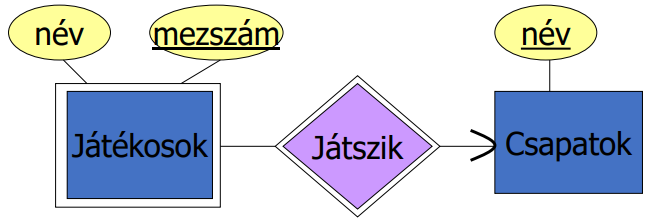
\includegraphics[width=0.3\linewidth]{EK-gyenge-egyedhalmaz}
\end{figure}

\pagebreak

\subsection{Tervezési technikák}

\begin{outline}
	\1 Redundancia elkerülése
		\2 Helypazarlás
		\2 Növeli az inkonzisztencia veszélyét
	\1 Gyenge egyedhalmazok óvatos használata
		\2 Általában jó, ha minden egyedhalmaznak van saját kulcsa
		\2 Saját kulcs készítése nem mindig lehetséges: nincs, ami kiosztaná ezeket (decentralizált rendszerek)
	\1 Attribútum használata egyedhalmaz helyett, ha lehetséges
		\2 Egyedhalmaz kell, ha ezek közül egy teljesül:
			\3 van legalább egy nem kulcs attribútum benne
			\3 egy "sok-egy" kapcsolatnak a "sok" végén szerepel
\end{outline}

\subsection{E/K diagrammból relációséma}

\begin{outline}
	\1 Egyedhalmazból reláció, attribútumból attribútum
	\1 Kapcsolatból reláció, aminek attribútumai:
		\2 összekapcsolt egyedhalmazok kulcsai
		\2 kapcsolat saját attribútumai

\begin{figure}[h!]
	\centering
	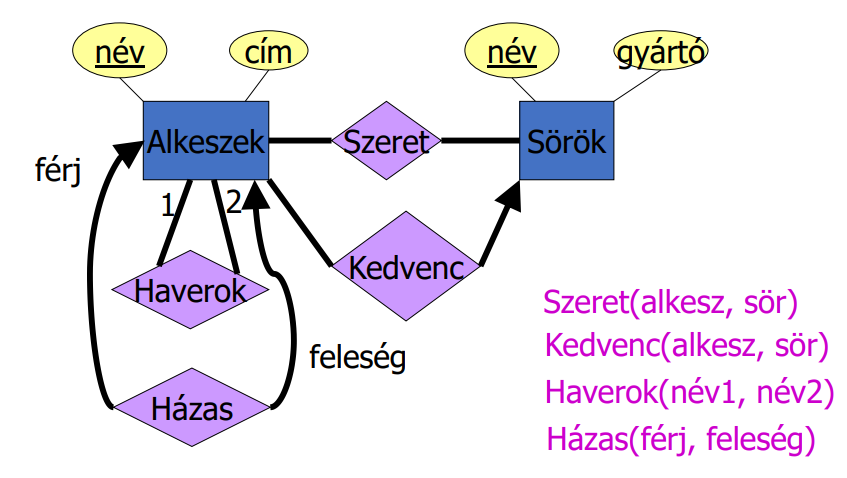
\includegraphics[width=0.4\linewidth]{EK-relációvá}
\end{figure}

	\1 Relációk összevonása: egyedhalmaz relációja összevonaható az egyedhalmazzal sok-egy kapcsolatban álló reláció, ha az eredeti egyedhalmaz a "sok", a másik pedig az "egy" oldalon van
		\2 Sok-sok kapcsolat összevonása helytelen, redundanciához vezet

\pagebreak

	\1 Gyenge egyedhalmazból reláció:
		\2 Relációnak a teljes kulcsot tartalmaznia kell.
		\2 Támogató kapcsolatokat nem írjuk át (redundanciához vezetne)
	\1 Alosztályok átalakítása
		\2 NULL értékek használata
			\3 Alosztály nem hoz be újabb relációt, csak újabb oszlopo(ka)t
			\3 Helytakarékos, kivéve, ha sok a NULL érték
			\3 Összekapcsolásokat is megspórolja
		\2 Objektumorientált megközelítés
			\3 Ősosztálynak és alosztálynak külön reláció
			\3 Ősosztály minden oszlopa létezik az alosztályban is
			\3 Egy egyed csak az egyik relációban van benne
			\3 Hasznos, ha az ősosztály nem-kulcs az alosztály oszlopait érintő lekérdezésekhez
		\2 E/K style
			\3 Ősosztálynak és alosztálynak külön reláció
			\3 Ősosztálynak csak a kulcs oszlopai léteznek az alosztály relációban
			\3 Egy egyed mindkét relációban benne van
			\3 Összekapcsolás szükséges, hogy minden adat egyszerre meglegyen
			\3 Hasznos, ha az alosztályt csak ritkán használjuk
\end{outline}

\pagebreak

\section{Objektum-relációs adatbázisok}

\subsection{Bevezetés}

\begin{outline}
	\1 Relációs és az objektumorientált modell egyesítése
		\2 OO modell komplexebb adattípusokat is támogat
		\2 Relációs modell magas szintű lekérdezéseket támogat
		\2 Objektum-relációs adatmodell ezt a kettőt akarja megtartani
	\1 Adatbázis-kezelő rendszerek (DBMS) fejlődése
		\2 OO rendszerek sokáig nem voltak elég hatékonyak
		\2 Relációs DBMS OO-val való kiterjesztése így jó megoldás volt
	\1 Főbb különbségek:
		\2 Attribútum típusa nem csak atomi típus lehet
		\2 Metódusok
		\2 Sorok egyéni azonosítót kapnak, lehet rájuk hivatkozást készíteni
\end{outline}

\subsection{Hivatkozások}

\begin{outline}
	\1 Cél: redundancia, módosítási anomáliák kiküszöbölése
		\2 Áttekinthetőbb alternatíva egy kapcsolási táblára
	\1 Hivatkozás típus rekurzívan van definiálva
	\1 A attribútum R sémájú sorra történő...
		\2 hivatkozás jelölés: A(*R)
		\2 hivatkozás halmaz (több sorra hivatkozás) jelölés: A(\{*R\})
	\1 Ha T egy UDT, akkor REF T egy hivatkozás (ami egy típus)
	\1 OID (objektum azonosító): beépített azonosító, alapból rejtett
	\1 Oracle: nincs különbség hivatkozás követés és normál mező elérés között
		\2 De ha \texttt{ff.sör} egy hivatkozás, akkor \texttt{SELECT DEEREF(ff.sör)} kell
	\1 SQL-99: ha \texttt{ff} egy reláció alias, akkor \texttt{ff.sör()->név}
	\1 Beszúrás: \texttt{SELECT típus(REF(<alias>), ... FROM ....} segítségével
\end{outline}

\subsection{Felhasználó által definiált adattípus: User Defined Type, UDT}

\begin{outline}
	\1 Hasonló OOP-hez: adatszerkezet és annak metódusai
	\1 Oracle: \texttt{CREATE TYPE <típusnév> AS OBJECT (<név-típus pár lista>);}
		\2 SQL szabvány: AS után nincsen OBJECT
	\1 1. felhasználási mód: sortípus: reláció ilyen adatokat tárol
		\2 Egy oszlop van a táblában, azon belül több mező
		\2 \texttt{CREATE TABLE <név> OF <UDT>;}
		\2 Lekérdezés: \texttt{SELECT <alias.xy> FROM <reláció> <alias>}
			\3 Oracle esetén az alias mindig kötelező
			\3 SQL-99 esetén \texttt{xy} helyett \texttt{xy()} (egy generátor) kell
		\2 Beszúrás
			\3 Oracle: sima \texttt{INSERT}, konstruktor hívással
			\3 SQL-99: mutátorok (\texttt{R.A(42)}) kellenek
				\4 Először létre kell hozni egy változót: \texttt{SET v = MyType();}
				\4 Utána mutálni kell: \texttt{v.x(42); v.y("valami");}
				\4 Végül be kell szúrni: \texttt{INSERT INTO MyTable VALUES(v);}
	\1 2. felhasználási mód: egy reláció attribútumának a típusa
\end{outline}

\pagebreak

\subsection{Metódusok UDT-ken belül}

\begin{outline}
	\1 Oracle:
		\2 CREATE TYPE-ban kell deklarálni, mint egy attribútumot:\\
		\texttt{MEMBER FUNCTION <név>(<paraméterek>) RETURN <típus>, <pragma>}
		\2 \texttt{PRAGMA RESTRICT\_REFERENCES(<metódus>, WNDS)}
			\3 WNDS jelentése: nem módosíthat, csak read-only
			\3 RNDS jelentése: ki sem olvassa az adatokat
		\2 Definíció: \texttt{CREATE TYPE BODY <típus> AS MEMBER FUNCTION <metódus>(...) RETURN <típus> IS BEGIN ... END; END;}
			\3 Paramétereknél itt már nem kell \texttt{IN/OUT}
		\2 Saját objektum: SELF
\end{outline}

\subsubsection{Rendező metódusok}

\begin{outline}
	\1 Ezek segítségével működik az \texttt{ORDER BY, WHERE} lekérdezésben
	\1 SQL-99: EQUAL, LESSTHAN (logikai visszatérési érték)
	\1 Oracle: bármelyik lehet rendező metódus, nincs kötelező neve
		\2 ORDER prefix kell MEMBER FUNCTION elé deklarációnál
		\2 Kötelező pragma-k: WNDS, RNDS, WNPF, RNPS
		\2 Visszatérési érték: szám (<0, =0, >0)
\end{outline}

\pagebreak

\subsection{Beágyazott táblák}

\begin{outline}
	\1 Lényeg: oszlop típusa egy táblázat
	\1 Séma típusú attribútum jelölés: AttrNév(AttrTag1, AttrTag2)
		\2 Emlékeztető: ez nem egy tuple/struct, hanem egy táblázat
	\1 Séma típus rekurzívan van definiálva (kiindulás: atomi típus)
	\1 Példa: Oktatók(név, TAJ, címek(város, utca), tárgyak(tárgynév, kód))
	\1 Csak Oracle szintaxist nézünk
	\1 Tábla típus létrehozása: \texttt{CREATE TYPE S AS TABLE OF T}
	\1 Beágyazott relációk tárolása Oracle-ben:
		\2 "Fő" tábla létrehozásakor megadni az oszlop-tábla hol legyen tárolva
		\2 \begin{verbatim}CREATE TABLE Gyártók (..., sörök SörTáblaTípus)
		NESTED TABLE sörök STORE AS SörTábla;\end{verbatim}
	\1 Beszúrás: tábla konstruktora, utána sorok felsorolása
	\1 Beágyazott tábla lekérdezése:
		\2 Minta sima érték lenne, csak egy listát kapunk vissza, mint "skalárt"
		\2 Több beágyazott tábla esetén descartes szorzat a beágyazott táblákra
	\1 Beágyazott táblán belüli lekérdezés
		\2 Hagyományos táblává alakítás: \texttt{TABLE(SELECT .. FROM ..) <alias>}
	\1 Beágyazott táblává alakítása (pl. beszúráshoz):\\
	\texttt{CAST(MULTISET(SELECT ...) AS <type>)}
\end{outline}

\pagebreak

\section{XML és XML/DTD sémák}

\subsection{Félig strukturált modellek (semi-structured data)}

\begin{outline}
	\1 Félig strukturált modellek: XML, JSON, ...
	\1 Félig strukturált
		\2 Motiváció: adatok rugalmas megjelenítése
		\2 Motiváció: dokumentumok átadása rendszerek (/adatbázisok) között
		\2 Információt ad arról, hogy mi a séma (magán az adaton felül)
	\1 Gráfként felfogható
		\2 Csúcsok: objektumok
		\2 Élek: kapcsolatok, címke a kapcsolat neve
		\2 Levél: atomi értékek
\end{outline}

\subsection{XML (Extensible Markup Language) bevezetés}

\begin{outline}
	\1 Kezdő deklarációs sor: \texttt{<?xml version="1.0" encoding="utf-8" ?>}
	\1 Tagek (jelölők): \texttt{<tag> ... </tag>}
		\2 Tetszőlegesen egymásba ágyazhatók
		\2 Üres tag: \texttt{<tag/>}
		\2 Érzékenyek a kis- és nagybetű különbségekre
	\1 Jól formált XML:
		\2 Önálló tagek bevezetése megengedett
		\2 Nem hiányzik a deklarációs sor
		\2 Minden nyitó tagnak van záró párja + jó sorrend, "helyes zárójelezés"
	\1 Valid XML: egy előre adott sémának megfelel, pl. DTD séma, XML séma
\end{outline}

\pagebreak

\subsection{XML felhasználása}

\begin{outline}
	\1 Információintegrációs probléma:
		\2 adatbázis modellek (relációs, NoSQL, stb) eltérnek
		\2 sémák eltérnek
		\2 más mértékegység, stb.
	\1 Régi, örökölt adatbázisokra támaszkodnak régi alkalmazások, ezeket meg akarjuk tartani
		\2 Megoldás: interfészt vezetünk be régi adatbázisok fölé
		\2 Új felhasználó az interfészen keresztül lép kapcsolatba az adattal
		\2 Az interfész közös több örökölt adatbázison
	\1 Integrációra két megközelítés: (mi legyen az interfész)
		\2 Adattárházba naponta/hetente szinkronizáció
			\3 Egy csomagoló adatbázisból adattárházba viszi az adatot
			\3 Egy irányú a megoldás: adattárházból nem lehet módosítani
				\4 Ez biztos?
		\2 Nézetek létrehozása, mintha integrált rendszer részei lennének
			\3 Mediátor csomagolókon keresztül beszél az adatbázisokkal
			\3 Két irányú a kapcsolat: lekérdezés és módosítás is lehet
\end{outline}

\pagebreak

\subsection{DTD séma}

\begin{outline}
	\1 Speciális formátumot használ (nem XML)
	\1 Felhasználás
		\2 <!DOCTYPE ...> a deklarációs sor és a dokumentum közé illeszthető
		\2 külön fájl: <!DOCTYPE kocsmák SYSTEM "bar.dtd">
	\1 Elemek: \texttt{<!ELEMENT <név> (alelemek...)}
		\2 Egy elemben lehet adat (levél, \texttt{\#PCDATA}) vagy elemek (vagy üres)
		\2 Üres elem: <!ELEMENT valami EMPTY> (tag: <valami <attr...>/>)
		\2 Alelemek megadása: típus és utána opcionálisan multiplicitás (*,+,?)
		\2 Alelemeknél van VAGY (|): \texttt{<!ELEMENT név ((x,y) | (a,b))>}
	\1 Attribútumok: \texttt{<!ATTLLIST Elem A1 Type1 Mod1 A2 Type2 Mod2...>}
		\2 "Mod": \#IMPLIED (opcionális), \#REQUIRED (kötelező)
			\3 \#DEFAULT (hogyan kell használni? nem hangzott el)
			\3 \#FIXED (mindig egy adott értéket kell megadni... valahogy)
		\2 Adattípusok: CDATA, ID, IDREF, IDREFS
			\3 CDATA: szöveg
			\3 ID, IDREF: egymásra mutathatnak az adatok, emiatt gráfot alkothatnak (nem pedig fát)
			\3 ID: azonos típusú elemnek nem lehet ugyan ilyen értéke (unique)
			\3 IDREF: nem tudjuk megmondani, hogy milyen típusú elemre mutasson
			\3 IDREFS: egyszerre többre hivatkozás
	\1 \begin{verbatim}
	<!DOCTYPE kocsmák [
	  <!ELEMENT kocsmák (kocsma*, sör*)>
	  <!ELEMENT kocsma (felszolgál+)>
	    <!ATTLIST kocsma név ID #REQUIRED>
	  <!ELEMENT felszolgál (#PCDATA)>
	    <!ATTLIST felszolgál melyikSör IDREF #REQUIRED>
	  <!ELEMENT sör EMPTY>
	    <!ATTLIST sör név ID #REQUIRED>
	    <!ATTLIST sör kapható IDREFS #IMPLIED>
	]>
	\end{verbatim}
\end{outline}

\pagebreak

\subsection{XML séma}

\begin{outline}
	\1 XML formátum, így az első sor: \texttt{<?xml version=... ?>}
	\1 Root tag: \texttt{<xs:schema xmlns:xs="URL"> ... </xs:schema>}
	\1 Felhasználás: <valami xmlns:xsi="schema-URL"\\
	xsi:noNamespaceSchemaLocation="valami.xsd"> ... </valami>
\end{outline}

\subsubsection{Egyszerű element (xs:element)}

\begin{outline}
	\1 Kötelező attribútum: name (tag neve)
	\1 Kötelező attribútum: type (érték típusa, pl. xs:string)
	\1 Nincs alelem
\end{outline}

\subsubsection{Összetett típusok (nem element, csak típus)}

\begin{outline}
	\1 Nem kötelező nevesíteni, lehet egyből egy xs:element aleleme (pl. ha csak egyszer használjuk)
	\1 Összetett (alelemet tartalmazó) típusok: xs:complexType
		\2 Kötelező attribútum: name (tag neve)
		\2 Típus: alelemek írják le
	\1 xs:sequence: xs:element sorozata
		\2 minOccurs és maxOccurs attribútumok minden xs:element-en
		\2 occurs értékek: szám (0,1,stb.) vagy unbounded
	\1 xs:attribute: name, type, use="required/optional" (alapból optional)
\end{outline}

\subsubsection{Megszorítás típusok (nem element, csak típus)}

\begin{outline}
	\1 Gyökér: xs:simpleType name=...
	\1 Alelem: \texttt{<xs:restriction base=típus> ... </xs:restriction>}
		\2 Típus: milyen típusú elemek lehetnek, mit szorítunk meg
		\2 \texttt{\{min/max\}\{Inclusive/Exclusive\}}: alsó/felső korlát megadása
	\1 Lehetséges elemek felsorolása: 1-1 \texttt{xs:enumeration value="..."} alelem
\end{outline}

\pagebreak

\subsubsection{Kulcsok}

\begin{outline}
	\1 xs:element-hez tartozhat xs:key alelem: \texttt{<xs:key name="..."> ...}
		\2 <xs:selector xpath="kocsma" />
		\2 <xs:field xpath="@nev" /> (@ jelentése: attribútum)
		\2 Jelentése: szelektor által megadott elemek adott field-jének mind unique-nak kell lennie
	\1 xs:element-hez tartozhat: \texttt{<xs:keyref name="..." refer="kulcs">}:
		\2 xs:key-hez hasonlóan selector és field beállítás kell
		\2 Jelentése: bizonyos értékeknek egy létező kulcsot kell leírniuk
\end{outline}

\begin{verbatim}
<?xml version = "1.0" encoding = "utf-8" ?>
<xs:schema xmlns:xs = "http://www.w3.org/2001/XMLSchema">
    <xs:complexType name = "sörTípus">
        <xs:attribute name = "név" type = "xs:string" use = "required" />
    </xs:complexType>
    <xs:complexType name = "kocsmaTípus">
        <xs:sequence>
            <xs:element name = "sör" type = "sörTípus"
                minOccurs = "1" maxOccurs = "unbounded" />
        </xs:sequence>
        <xs:attribute name = "név" type = "xs:string" use = "required" />
    </xs:complexType>
    <xs:complexType name = "kocsmákTípus" >
        <xs:sequence>
            <xs:element name = "kocsma" type = "kocsmaTípus"
                minOccurs = "0" maxOccurs = "unbounded" />
        </xs:sequence>
    </xs:complexType>
    <xs:element name = "kocsmák" type = "kocsmákTípus" />
</xs:schema>
\end{verbatim}

\pagebreak

\section{XML lekérdezőnyelvek}

\begin{outline}
	\1 XPath/XQuery adatmodell
		\2 Tételek listájával (item sequence) dolgozunk: ez a bemenet, kimenet
		\2 Tétel lehet: egyszerű (levél, skalár érték) vagy csomópont
	\1 Csomópontok:
		\2 dokumentum csomópont: teljes dokumentum (pl. doc(http://...))
		\2 elem csomópont: xml tag és az alelemei
		\2 attribútum
\end{outline}

\subsection{XPath}

\begin{outline}
	\1 Emlékeztető: eredmény mindig egy lista
	\1 Tag-ek követése: /kocsmák/kocsma/ár (alemeket járunk be sorban)
	\1 Attribútum hivatkozása: @ prefix
	\1 Nem csak a gyökérből lehet indulni:
		\2 //X/... a dokumentumban bárhol (gyökérben vagy lejjebb) lévő X tag-től indul
		\2 Eredmény sorrendben lesz: feljebb (pl. gyökérből) induló esetek lesznek először
		\2 Nem csak gyökér szinten lehet alkalmazni, hanem lejjebb is
	\1 Tetszőleges tag: * (pl. /*/*/ár)
	\1 Feltételek: tag után [...]
		\2 Atomi értékű törzsre szűrés: [text()]
		\2 Szám összehasonlítás: [. < 3.14] \;\; (. az aktuális elem)
		\2 Attribútum megszorítás: [@valami = "xyz"]
\end{outline}

\pagebreak

\begin{outline}
	\1 Tengelyek (axes): következő lépésnél feldolgozandóak listája
		\2 Alapértelmezett: \texttt{child::} (pl. /child::kocsmák)
		\2 attribute:: (@ hosszú formája)
		\2 parent:: (pl. //könyv/cím[. = 'Valami']/parent::könyv)
		\2 descendant-or-self:: (hasonló a //-hez)
		\2 ancestor::, ancestor-or-self::
		\2 self:: (. hosszú formája)
\end{outline}

\section{XQuery}

\begin{outline}
	\1 Nem vettük, nem maradt rá idő
\end{outline}

\pagebreak

%EA - GYAK ELVÁLASZTÓ

\section{Relációs algebra gyakorlati jegyzet}

\begin{outline}
	\1 $\sigma_{x=NULL}$ az nem része az alap algrebrának, csak a kiterjesztett algebrának
	\1 Relációs algebra mindig átírható SQL-be, de visszafelé nem
		\2 pl. alkérdések nincsenek relációs algebrában
	\1 Tábla indexelve: átnevezés, csak így könnyebb (hivatalosan: $\rho_{Sz_1}(Sz)$)
	\1 Min két gyümölcsöt szeret: $Sz_1 \times Sz_2$, 1 sorban 2 különböző gyümölcs
	\1 Gyakorlaton $\rightouterjoin$ helyett $\bowtie_R$ jelet használjuk (teljes: $_L \bowtie_R$)
	\1 Komplementer halmaz képzés: $( \Pi_{name}(SZ) \times \Pi_{fruit} (SZ) ) \setminus (SZ)$
	\1 Tábla nevét $\bowtie$-nál mindig ki kell írni, kivéve, ha NATURAL JOIN van
\end{outline}

\subsection{Kiterjesztett algebra}

\begin{outline}
	\1 Multihalmazzal dolgozunk
	\1 Létezik NULL érték
	\1 Csoportképzés (group by féleség): $\gamma$ (gamma)
		\2 GROUP BY X, COUNT(Y) AS db: $\gamma_{X,COUNT(Y) \to db} (R)$
		\2 Aggregációs függvények: MIN, MAX, SUM, AVG, COUNT
		\2 Ezután csak az alsó indexben lévőket lehet használni
		\2 Lehet 0/1/több oszlop alapján group-olni, lehet 0/1/többet aggregálni
		\2 Relációs algebrában nincs külön WHERE ÉS HAVING (csak $\sigma$)
		\2 Relációs algebrában is van COUNT(*)
		\2 COUNT(DISTINCT X) = COUNT($\delta$ X)
	\1 Sorba rendezés: $\tau$ (tau), ORDER BY X: $\tau_{X} (R)$
\end{outline}

\pagebreak

\section{SQL függvények, műveletek}

\begin{outline}
	\1 Dátum, idő
		\2 TO\_DATE('2000-01-01', 'YYYY-MM-DD') -> dátum
		\2 TO\_CHAR(DATE, 'YYYY-MM-DD') -> szöveg
		\2 SYSDATE -> aktuális dátum \;\;\; (NEM FÜGGVÉNY)
		\2 Dátumok kivonása a napok számát adja meg
	\1 Szöveg (string) kezelés
		\2 Oracle 1-től indexel
		\2 SUBSTR('valami', 2, 1) -> a
		\2 SUBSTR('valami', -2, 1) -> m
		\2 SUBSTR('valami', 2) -> 'alami'
		\2 LENGTH('alma') -> 4
		\2 INSTR('valami', 'a', 1, 2) -> 2. 'a' pozíciója az 1-es index után
		\2 RPAD('a', 4, '\#') -> 'a\#\#\#', LPAD, üres szöveget nem lehet
		\2 UPPER('alma') -> 'ALMA', LOWER
		\2 mezo (NOT) LIKE '\_I\%' -> 2. betű I, hossza >= 2
		\2 Konkatenáció: \texttt{'a' || 'b'}
	\1 Matematika
		\2 ROUND(0.123, 2) -> 0.12
		\2 SQRT(x), FLOOR(x), CEIL(x)
		\2 MOD(x, 2)
		\2 LEAST(a, b), GREATEST(a, b)
	\1 NVL(NULL, 'Ismeretlen', ...) -> első nem-NULL érték
	\1 TO\_NUMBER('42') és TO\_CHAR(42)
\end{outline}

\pagebreak

\section{PL/SQL (PL SQL, PLSQL) programozás}

\subsection{Függvény, procedura létrehozás}

\begin{outline}
	\1 Sql Developer buta és nem ismeri fel, hogy hol ér véget a fv
		\2 Tehát ki kell jelölni a fv-t és csak az fv-t és úgy futtatni
	\1 \begin{verbatim}
CREATE OR REPLACE PROCEDURE <név> (params...) IS
    <változó> <típus> [:= kezdőérték];
  BEGIN
    ... --Minden sor végén ;
  END [név];
	\end{verbatim}
		\2 Hívása: CALL <név>(params...);
	\1 \begin{verbatim}CREATE OR REPLACE FUNCTION <név> (params...) RETURN <típus> IS ...\end{verbatim}
		\2 Hívás: SELECT <név>(params1), <név>(params2) FROM dual;
	\1 Paraméterek: pl. [IN] [OUT] nev VARCHAR2 (nincs méret!)
		\2 IN (bemeneti): alapból minden ez, nem lehet módosítani
		\2 IN OUT: konstans nem adható át ennek
\end{outline}

\subsection{Nyelvi konstrukciók}

\begin{outline}
	\1 For ciklus: FOR i IN 1..n LOOP ... END LOOP;
		\2 Másik irányban: ... IN REVERSE ...
	\1 While ciklus: WHILE n > 0 LOOP ... END LOOP;
	\1 IF <felt> THEN ... [ELSIF <felt> THEN ...] [ELSE ...] END IF;
	\1 Loop-ból kilépés: \texttt{EXIT WHEN ...}
	\1 Early "return": \texttt{IF ... THEN CONTINUE; END IF;}
\end{outline}

\pagebreak

\subsection{Egyéb tudnivalók, trükkök}

\begin{outline}
	\1 \begin{verbatim}dbms_output.put_line('Hello' || 'nev'); --debug msg\end{verbatim}
		\2 Be kell kapcsolni: \texttt{SET SERVEROUTPUT ON} (egy ideig hat)
	\1 Név nélküli blokk, függvény hívás egyszerűen:\\
	\texttt{DECLARE n := 42; BEGIN test(n); END;}
	\1 Szöveg típus: \texttt{VARCHAR2}, ami üres esetén \texttt{NULL}
		\2 Általában nem baj, ha a függvényünk ilyen bemenetre nem működik
		\2 Ha üreshez akarunk konkatenálni, lehet érdemes inkább \texttt{VARCHAR1}
	\1 Tábla másolás, extra oszlop létrehozásávál:\\
	\texttt{CREATE TABLE ... AS SELECT dolgozo.*, 1 sorszam FROM dolgozo;}
\end{outline}

\subsection{Adat bekérés, prompt, \texttt{ACCEPT}}

\begin{outline}
	\1 Egy makró-t töltünk fel (ami egy C-s \verb|#define| féleség)
	\1 Hasznos ZH-n név nélküli blokkok tesztelésére
	\1 \texttt{ACCEPT <név> <típus> PROMPT 'Popup prompt szöveg';}
	\1 Makró használat: \texttt{\&<név>}
		\2 Ha makró szöveg volt, attól még idézőjelek nincsenek ebben benne
		\2 Ilyenkor használat: \texttt{'\&<név>'}
	\1 \texttt{ACCEPT} sor nélkül is jó, de ekkor minden futtatáskor bekéri az értékét
\end{outline}

\pagebreak

\subsection{Kurzorok (\texttt{CURSOR})}

\begin{verbatim}
	CREATE OR REPLACE PROCEDURE teszt IS
	  CURSOR curs1 IS SELECT * FROM SZ;
	  rec curs1%rowtype; --1. lehetőséghez kell
	BEGIN
	  --1. lehetőség: bonyolult, több kurzoros feladatra is jó
	  OPEN curs1;
	  LOOP 
	    FETCH curs1 INTO rec;
	    EXIT WHEN curs1%NOTFOUND;
	    -- valami(rec.adattag);
	  END LOOP;
	  CLOSE curs1;
	  
	  --2. lehetőség, nem kell a fenti 'rec' deklaráció
	  FOR rec IN curs1 LOOP
	    -- valami(rec.adattag);
	  END LOOP;
	END;\end{verbatim}

\subsubsection{Kurzorok módosításra}

\begin{outline}
	\1 Deklarálás: \texttt{CURSOR curs1 IS ... FOR UPDATE;}
		\2 UPDATE: akár delete-elni is lehet, nincs köze az UPDATE kulcsszóhoz
	\1 Lehet több olvasó, de egyszerre csak 1 író (és írás kizárja az olvasást)
		\2 \texttt{FOR UPDATE} nélküli eljárásban hívhatunk meg módosító eljárást
	\1 Cache-elt ResultSet-en iterálunk: iterálás közbeni változtatás nem látszik
	\1 Változtatás SQL-lel: \texttt{UPDATE ... SET ... WHERE CURRENT OF curs1;}
		\2 \texttt{rec} és tábla módosítása nem módosítja egymást
		\2 Manuálisan frissíthetjük a \texttt{rec}-et, majd azzal a táblát
	\1 Kapcsolt táblán iterálás, egyiken módosítás:
		\2 \texttt{FOR UPDATE} helyett \texttt{FOR UPDATE OF <oszlopnév...>}
		\2 Ez teljes zárat ad a táblára, nem csak az oszlopra (törölni is lehet)
	\1 Módosító \texttt{FUNCTION}-t \texttt{SELECT} helyett név nélküli blokkban futtatunk
\end{outline}

\pagebreak

\section{Példák}

\subsection{Tábla létrehozás}

\begin{verbatim}
DROP TABLE teszt_1;
CREATE TABLE teszt_1 (
  lebego REAL NOT NULL,
  egesz INT DEFAULT 0,
  nev VARCHAR2(100) UNIQUE,
  CONSTRAINT pk_teszt_1 PRIMARY KEY (egesz, nev)
);

DROP TABLE teszt_2;
CREATE TABLE teszt_2 (
  datum DATE PRIMARY KEY
);

DROP TABLE teszt_3;
CREATE TABLE teszt_3 (
  egesz INT,
  nev VARCHAR2(100),
  datum DATE REFERENCES teszt_2 (datum),
  CONSTRAINT fk_teszt_1 FOREIGN KEY (egesz, nev)
                        REFERENCES teszt_1 (egesz, nev)
);
\end{verbatim}

\pagebreak

\subsection{PL/SQL függvény}

\begin{verbatim}
CREATE OR REPLACE FUNCTION faktor(n INTEGER) RETURN INTEGER IS
  val INTEGER := 1;
BEGIN
  FOR i IN 2..n LOOP
    val := val * i;
  END LOOP;
  RETURN val;
END;
SELECT faktor(0), faktor(5) FROM dual;
\end{verbatim}

\subsection{PL/SQL eljárás}

\begin{verbatim}
CREATE OR REPLACE PROCEDURE paratlan IS
  CURSOR curs1 IS SELECT * FROM dolgozo ORDER BY dnev;
  sorszam INT := 0;
BEGIN
  FOR rec IN curs1 LOOP
    sorszam := sorszam + 1;
    IF MOD(sorszam, 2) = 1 THEN
      dbms_output.put_line(TO_CHAR(sorszam) || '.: Név: '
          || rec.dnev || ', fizetés: ' || TO_CHAR(rec.fizetes));
    END IF;
  END LOOP;
END;
SET SERVEROUTPUT ON;
CALL paratlan();
\end{verbatim}

\end{document}
